\section{Fuzzy clustering}
%La clusterizzazione fuzzy, nota anche come soft k-means, è una tecnica avanzata di analisi dei dati che consente ai punti dati di appartenere a più di un cluster. Questa modalità differisce dalla tradizionale clusterizzazione "hard", dove ogni punto dati è assegnato esclusivamente a un singolo cluster, utilizzando invece una logica fuzzy per determinare l'appartenenza di un dato a ciascun cluster. In altre parole, anziché avere un'affermazione binaria di appartenenza (1 o 0), si ha una misura continua di appartenenza che varia da 0 a 1. Questo è espresso attraverso una funzione di similarità, $\mu_x(C)$, che rappresenta il grado di appartenenza di un dato $x$ a un cluster $C$.
Fuzzy clustering, also known as soft \gls{kmeans}, is a data analysis technique that allows data points to be assigned to more than one cluster. To understand this, it is important to define the concepts of a cluster, a centroid, and the distinction between hard and soft clustering. A cluster is a group of data points that share similar characteristics or are close to one another in a defined feature space. For example, in a two-dimensional space, a cluster might represent a dense grouping of points around a specific region. A centroid is the representative point of a cluster, often located at its geometric center or computed as the mean of all the points within the cluster.

\noindent In hard clustering, each data point is assigned exclusively to a single cluster, resulting in binary membership (i.e., a data point either belongs to a cluster or it does not). A common example is traditional \gls{kmeans} clustering. In contrast, soft clustering allows data points to have degrees of membership in multiple clusters. Instead of binary membership ($0$ or $1$), fuzzy clustering employs a continuous measure of membership that ranges from $0$ to $1$. This is represented by a similarity function, $\mathds{1}_C(x)$, which quantifies the degree to which a data point $x$ belongs to a cluster $C$.


% referenza K-Means
%La clusterizzazione fuzzy ha le sue radici nel lavoro di J.C. Dunn, che nel 1973 ha introdotto questo concetto come un'estensione dell'algoritmo di clustering k-means. Dunn ha evidenziato la maggiore precisione e robustezza della clusterizzazione fuzzy rispetto alla clusterizzazione rigida, soprattutto nella gestione dei dati anomali (outlier) \citep{FuzzyClustering_developDoc}.

\noindent Fuzzy clustering originated from the work of \citeauthor{FuzzyClustering_developDoc}, who introduced this concept as an extension of the \gls{kmeans} clustering algorithm in \citeyear{FuzzyClustering_developDoc}. \citeauthor{FuzzyClustering_developDoc} emphasized the increased accuracy and robustness of fuzzy clustering compared to hard clustering, particularly in handling anomalous data (outliers) \citep{FuzzyClustering_developDoc}.

\noindent The robustness of fuzzy clustering comes from its use of continuous membership degrees, which allows data points to partially belong to multiple clusters. This reduces the impact of outliers by assigning them smaller membership values across clusters, diluting their influence. In addition, fuzzy clustering better models overlapping clusters by capturing the uncertainty in their boundaries, a common feature in real-world data.

% membership function
%L’algoritmo proposto da Dunn è detto Fuzzy C-Means Clustering (FCM) e si basa sull’utilizzo della tecnica Expectation-Maximization (EM) per definire la funzione di appartenenza ai cluster. Questa tecnica è un approccio iterativo per la stima dei parametri statistici, come ad esempio i centroidi dei cluster. Il processoEM si articola in due fasi principali:
%\begin{enumerate}
%    \item Expectation (E): In questa fase, viene formulata una funzione di verosimiglianza che esprime la probabilità che un dato appartenga a ciascun cluster in base alla sua distanza o similarità rispetto ai centroidi.
%    \item Maximization (M): Nella fase di massimizzazione, vengono individuati i parametri dei modelli che massimizzano la verosimiglianza, in questo caso i centroidi dei cluster, tramite un procedimento di ottimizzazione.
%\end{enumerate}
\noindent The algorithm proposed by \citep{FuzzyClustering_developDoc} is known as the \gls{fcm} and employs the \gls{em} technique to define the cluster membership function. This method is an iterative approach for estimating statistical parameters, such as cluster centroids. The \gls{em} process consists of two main steps:
\begin{enumerate}
    \item Expectation (E): In this phase, a likelihood function is formulated. This function expresses the probability that a data point belongs to each cluster, based on its distance or similarity to the centroids.
    \item Maximisation (M): In the maximization phase, an optimization procedure is used to identify the model parameters that maximize the likelihood, specifically the centroids of the clusters.
\end{enumerate}

%In sintesi, la clusterizzazione fuzzy offre una maggiore flessibilità rispetto alla clusterizzazione rigida, consentendo una rappresentazione più accurata e dettagliata dei dati, soprattutto in presenza di dati eterogenei o outlier.
\noindent In summary, fuzzy clustering provides greater flexibility compared to hard clustering, allowing for a more accurate and detailed representation of the data, particularly in the presence of heterogeneous data or outliers.

\subsection{Insights}
%Per comprendere appieno l'algoritmo \gls{fcm}, si definiranno preliminarmente i concetti fondamentali su cui si basa.
To fully understand the \gls{fcm} algorithm, we must first define the fundamental concepts on which it is based.

%\noindent I "punti dati" sono le osservazioni o le entità nel nostro insieme di dati, ognuna caratterizzata da una serie di attributi o feature. Questi punti dati possono essere visti come punti nello spazio multidimensionale, dove ogni dimensione corrisponde a un attributo specifico.
\noindent \textbf{Data points}: These are the observations or entities in our dataset, each characterised by a set of attributes or features. Data points can be viewed as points in a multidimensional space, where each dimension corresponds to a specific attribute. To represent these points mathematically, each attribute is assigned a numerical value, resulting in a vector in $\mathbb{R}^K$, where $K$ is the number of attributes. For example, if an observation is described by three attributes height, weight and age, it can be represented as a vector $(h,w,a)\in\mathbb{R}^3$, where $h$,$w$,$a$ are numerical values corresponding to these attributes. This transformation from abstract attribute spaces to real-valued vectors enables the application of mathematical and computational techniques, such as clustering.

%\noindent Una volta che abbiamo definito i punti dati, possiamo procedere a organizzarli in gruppi chiamati "cluster". Un cluster è una raccolta di punti dati che condividono caratteristiche simili tra loro. L'obiettivo dell'algoritmo di clustering è quello di raggruppare i punti dati in modo che quelli all'interno dello stesso cluster siano più simili tra loro rispetto a quelli in cluster diversi.
\noindent \textbf{Clusters}: Once we have defined the data points, we can organize them into groups called clusters. A cluster is a collection of data points that share similar characteristics. The goal of the clustering algorithm is to group data points so that those within the same cluster are more similar to each other than to those in different clusters.

%\noindent Ogni punto dati può essere associato a uno o più cluster attraverso la funzione di appartenenza a un cluster, indicata con $\mu_x$. Questa funzione assegna a ciascun punto dati un grado di partecipazione a ciascun cluster, rappresentato da un valore compreso tra $0$ e $1$. Ad esempio, se $\mu_x(C) = 1$, significa che il punto dati $x$ appartiene completamente al cluster $C$, mentre se $\mu_x(C) = 0.5$, significa che $x$ appartiene al cluster $C$ con una certa incertezza o ambiguità.
\begin{modified}
\noindent \textbf{Cluster Membership Function}: Each data point can be associated with one or more clusters through the cluster membership function, denoted as $\mathds{1}_C(x)$, where $x$ represents a specific data point and $C$ represents a cluster. This function assigns each data point a degree of membership in each cluster, represented by a value between $0$ and $1$. For example, if $\mathds{1}_C(x) = 1$, it indicates that data point $x$ belongs completely to cluster $C$. Conversely, if $\mathds{1}_C(x) = 0.5$, it suggests that $x$ has some degree of uncertainty or ambiguity in its membership to cluster $C$.
\end{modified}
\begin{notation}
Denote:
\begin{itemize}
\item the dataset with \\ $\mathcal{S} = (x_i)_{i=1:N}$ where $x_i\in\mathbb{R}^K$
\item the set of cluster centroids with \\ $\mathcal{C}={C_1,\dots,C_M}$ where $C_j\in\mathbb{R}^K$ with centroids $c_1,\dots,c_M$
\item the measure of the membership of a data point $x_i$ in the cluster $C_j$ with \\ $\mathds{1}_{C_j}(x_i)\in\left[0,1\right]$
\item the weight matrix with \\ $U=(u_{ij})$ where $u_{ij}=\mathds{1}_{C_j}(x_i)$
\item the quadratic Euclidean distance matrix with \\ $D^2=(d^2_{ij})$ where $d_{ij}^2=\|x_i-c_j\|^2$
\end{itemize}
\end{notation}
\newpage
\begin{exempli_gratia}
To understand the meaning of data points and clusters, let us consider the following example:

\noindent Imagine we need to classify the apples transported by a lorry into two color categories: green and red. However, within this set, there might also be yellow apples. The $k$-means algorithm would treat a yellow apple as an anomaly compared to the red and green apples. In contrast, fuzzy clustering quantifies this anomaly by asserting that a yellow apple is a blend of red and green.

\noindent The colours of the apples can be represented in a one-dimensional space. In this space, we observe a distribution of data points showing green and red at the extremes, with yellow apples located in the center.

\noindent Clusters, in the context of fuzzy logic, are sets defined by centroids representing specific shades of colour, which are not necessarily present in the set of data points. For example, if there are red and green apples, there are actually two centroids representing specific shades of red and green, even though there are no apples with such colour shades.

\begin{center}
	
\includegraphics[width=0.5\linewidth]{Figures/apple.png}
\end{center}
\end{exempli_gratia}

\begin{remark}
	The \gls{fcm} algorithm recognizes that real-world data may contain errors or uncertainties. Instead of rigidly assigning each data point to a single cluster, it introduces a measure of uncertainty in the assignment. This approach results in assigning a fuzzy degree of membership to each point concerning each cluster, rather than relying on a binary classification.
\end{remark}
\newpage
\begin{definition}[membership measure]\label{def:fuzzy}
	Given a point $x$ and a cluster $c$, the membership measure $\mathds{1}_c(x)$ is a probability distribution proportional to the inverse of the square of the Euclidean distance between the point $x$ and the centroid of the cluster $c$, i.e. $\frac{1}{\|x-c\|^2}$.\\ In other words:
	$$\forall x \left( \sum_{C\in\mathcal{C}}\mathds{1}_C(x)=1 \right) \quad \text{and} \quad \forall x \, \exists \lambda_x \, \forall j=1:M \left(\mathds{1}_{C_j}(x)=\frac{\lambda_x}{\|x-c_j\|^2}\right)$$

		\bigskip\noindent Consequently:
		\[
			\forall x \, \exists \lambda_x \left( 1 = \sum_{C\in\mathcal{C}}\mathds{1}_C(x) = \sum_{j=1}^M\frac{\lambda_x}{\|x-c_j\|^2} = \lambda_x\sum_{j=1}^M\frac{1}{\|x-c_j\|^2}\right)
		\]
		So for all $x$ it holds that $\lambda_x = \frac{1}{\sum_{j=1}^M\frac{1}{\|x-c_j\|^2}}$

		\bigskip\noindent Finally:
		\begin{align*}
			u_{ij} &= \mathds{1}_{C_j}(x_i) = \frac{\lambda_{x_i}}{\|x_i-c_j\|^2} = \frac{\frac{1}{\sum_{k}\frac{1}{\|x_i-c_k\|^2}}}{\|x_i-c_j\|^2} \\
			&= \frac{\frac{1}{\|x_i-c_j\|^2}}{\sum_{k}\frac{1}{\|x_i-c_k\|^2}} = \frac{\frac{1}{d_{ij}^2}}{\sum_{k}\frac{1}{d_{ik}^2}} = \frac{1}{\sum_{k}\frac{d_{ij}^2}{d_{ik}^2}}
		\end{align*}
\end{definition}

\paragraph{The objective function}
	As already mentioned, the algorithm \gls{fcm} can be seen as a derivation of \gls{kmeans}. To better understand this step, we will explain what \gls{kmeans} is.

	\noindent The \gls{kmeans} algorithm is one of the most widely used clustering methods in data analysis. It divides a data set into a predefined number $M$ of clusters, each represented by a centroid. The algorithm iteratively refines the cluster assignments and centroids to minimise the intra-cluster variance. In other words, the goal of the \gls{kmeans} algorithm is to minimise the sum of the variances of all clusters, which is defined as the sum of the squared distances between each point in the cluster and the cluster centroid.

	\noindent Formally, the goal of the \gls{kmeans} algorithm is to solve this problem over \\ $\mathcal{C} = \{C_1,\ldots,C_M\}$, with $C_j\subseteq\mathcal{S}\forall j$:
	\begin{equation*}
		\text{argmin}_\mathcal{C}\left[\sum_{j=1}^M\sum_{x \in C_j}\|x-c_j\|^2\right]
	\end{equation*}
	where $\forall x \exists!j : x\in C_j$.

	\noindent The \gls{kmeans} algorithm assigns each data point to a single cluster $C_j$ in a "hard" way, meaning that each point belongs exclusively to one cluster. The \gls{fcm} algorithm generalises this approach by replacing the binary assignment of points with a continuous membership function, $\mathds{1}_C(x)$, which quantifies the degree to which a data point belongs to each cluster.

	\noindent In the case of fuzzy clustering, the membership of a point in a cluster is expressed by a fuzzy measure instead of a Boolean logic. The objective function of the \gls{kmeans} method can be rewritten equivalently with membership measures:
	\begin{equation*}
		\sum_{C\in\mathcal{C}}\sum_{x \in \mathcal{S}}\mathds{1}_C(x)\|x-C\|^2
	\end{equation*}
	where $\mathds{1}_C(x)$ represents the membership measure of point $x$ in cluster $C$ ($1$ if $x\in C$, $0$ otherwise).
	\begin{modified}This objective function reflects the weighting of the squared distances by the membership measure of each point in the clusters.
	\end{modified}

\begin{definition}[Loss function and cluster weight]\label{def:fuzzyloss}
	We define the fuzzy clustering loss function from the \gls{kmeans} algorithm as follows:
	\begin{equation}
		L_\mathcal{S}(\mathcal{C}) := \sum_{C\in\mathcal{C}}p_\mathcal{S}(C) := \sum_{C\in\mathcal{C}}\sum_{x \in \mathcal{S}}\mathds{1}_C(x)^2\|x-c\|^2
		\label{eq:loss}
	\end{equation}
	\noindent where $p_\mathcal{S}(C)$ is the weighted sum of the squared distances between the points in the cluster $C$ and its centroid. This loss function is coercive on the centroids, which means that it tends to infinity when the centroids recede to infinity, and has a finite lower bound when the centroids are bound to a compact set in the data space. Formally, for any norm defined over $\vec{\mathcal{C}}$, a vector representation of $\mathcal{C}$ with $M\times K$ components, it hold that:
	\begin{equation*}
		\lim_{\|\vec{\mathcal{C}}\|\to\infty} L_\mathcal{S}(\mathcal{C}) = \infty
	\end{equation*}
	and
	\begin{equation*}
		L_\mathcal{S}(\mathcal{C}) \geq 0
	\end{equation*}
	For this reason we know that there is a global minimum although the uniqueness of local minima is not guaranteed.\footnote{for more about coercitive functions, see \\ \url{https://www1.mat.uniroma1.it/people/lanzara/OTT0708/Ottimizzazione0708.pdf}}
\end{definition}

\paragraph{EM} As previously mentioned, the \gls{kmeans} and \gls{fcm} algorithms can be seen as applications of the EM technique. Specifically, in the case of the \gls{kmeans} algorithm, the procedure can be summarized as follows:
\begin{itemize}
	\item \textbf{E-step (Expectation)}: Each data point is assigned to the nearest centroid. For example, a yellow apple would be assigned to a red apple rather than a green apple. This corresponds to a "hard" assignment, where each data point is exclusively linked to one cluster. This step defines the membership measure and the corresponding optimization problem:\\ $\text{argmin}_\mathcal{C}\left[\sum_{C\in\mathcal{C}}\sum_{x \in C}\|x-c\|^2\right]$
	 \item \textbf{M-step (Maximization)}: With fixed memberships, the centroids are recomputed by solving the optimization problem. Specifically, it can be shown that:\\ $C = \text{mean}\left[x\middle|x\in C\right] = \frac1{|C|}\sum_{x\in C} x$
\end{itemize}
\noindent Both steps alternate iteratively: the \textbf{E-step} minimises the loss function \\ $\sum_{C\in\mathcal{C}}\sum_{x \in C}\|x-c\|^2$ for fixed centroids, and the \textbf{M-step} minimises the same loss function for fixed memberships. Thus, the \gls{kmeans} algorithm minimises the loss function through an alternating optimization approach.

\noindent The \gls{fcm} algorithm is similar:
\begin{itemize}
	\item \textbf{E-step (Expectation)}: The membership matrix $U$ is computed as defined in \cref{def:fuzzy}, assigning each data point a degree of membership between $0$ and $1$. This corresponds to a "soft" assignment, where each point can belong to multiple clusters with varying degrees of membership. This step defines the membership measure and the corresponding optimization problem:\\ $\text{argmin}_\mathcal{C}\left[\sum_{C\in\mathcal{C}}\sum_{x \in \mathcal{S}}\mathds{1}_C(x)^2\|x-c\|^2\right]$
	\item \textbf{M-step (Maximization)}: With fixed memberships, the centroids are recomputed by solving the optimization problem to minimize the objective function.
\end{itemize}

\bigskip\noindent Now we compute the solution of objective function of \gls{fcm} algorithm during '\textbf{M-step}' phase.
\begin{theorem}[Update formula 'M']
	\label{thm:Mupdate}
    Given the matrix $U$, the loss function of \cref{eq:loss} reaches its minimum when the centroids are given by:
    \begin{equation}
        c^{\texttt{new}}_j = \frac{\sum_{i=1}^Nu_{ij}^2x_{i}}{\sum_{i=1}^Nu_{ij}^2} \text{\hspace{1cm}} \forall j
    \end{equation}
	\begin{proof}
	    Given the matrix $U$, the loss function is differentiable, convex and coercive. Consequently, to find the global minimum of the function, it is sufficient to find the points where the gradient is null.

	    \noindent Calculating the partial derivatives of the gradient with respect to the centroids $c_j$, we obtain:
	\begin{equation*}
	    \frac{\partial}{\partial c_{j}} L_\mathcal{S}(\mathcal{C}) = \frac{\partial}{\partial c_{j}} p_\mathcal{S}(c_j) = \sum_{i=1}^N\frac{\partial}{\partial c_{j}} u_{ij}^2\|x_i-c_j\|^2 = 2\sum_{i=1}^N u_{ij}^2\left(c_{j}-x_{i}\right)
	\end{equation*}

	\noindent The gradient is null when all partial derivatives are null, which implies:
	\begin{equation*}
	    \sum_{i=1}^N u_{ij}^2c^{\text{new}}_{j} = \sum_{i=1}^N u_{ij}^2x_{i} \quad \forall j
	\end{equation*}

	\noindent Since $c^{\text{new}}_j$ does not depend on the index $i$, the thesis is proved.
	\end{proof}
\end{theorem}

\noindent The \gls{kmeans} algorithm uses the \gls{em} technique to optimally select centroids and memberships. Similarly, \gls{fcm} replaces hard assignments with soft ones, as formalized in the following theorem.\newpage

\begin{theorem}[Update formula '\textbf{E}'] \label{thm:Eupdate}
	Let \(\mathds{1}^\star\) be the solution of the optimization problem in the '\textbf{E-step}' for fixed centroids \(\mathcal{C}\):
	\[
	\textnormal{argmin}_{\mathds{1}}\left[\sum_{C\in\mathcal{C}}\sum_{x \in \mathcal{S}}\mathds{1}_C(x)^2\|x-c\|^2\right].
	\]
	Updating the membership matrix \(U\) provides the optimal solution:
	\[
	u_{ij} = \mathds{1}^\star_{C_j}(x_i).
	\]
\begin{proof}
	Since the membership degrees $\mathds{1}_C(x)$ are independent for different data points $x\in \mathcal{S}$, the optimization problem can be decoupled into independent subproblems for each cluster.
	$$\textnormal{argmin}_{ \mathds{1}}\left[\sum_{C\in\mathcal{C}}\sum_{x \in \mathcal{S}}\mathds{1}_C(x)^2\|x-c\|^2\right] = \sum_{x\in\mathcal{S}}\textnormal{argmin}_{ \mathds{1}}\left[\sum_{c \in \mathcal{C}}\mathds{1}_C(x)^2\|x-c\|^2\right]$$

	\noindent The optimization problem $\textnormal{argmin}_{\mathds{1}}\left[\sum_{c \in \mathcal{C}}\mathds{1}_C(x)^2\|x-c\|^2\right]$ is a convex quadratic problem (QP) because the loss function is quadratic, and the feasible region is a convex set (probability simplex). The solution can thus be found using the \gls{kkt} conditions.

	\bigskip \noindent In general, these kinds of problems are solved mechanically through the conditions \gls{kkt}, stated below:

	\itshape\noindent Consider the following nonlinear optimisation problem in standard form:
	$$\textnormal{argmin}_x f(x)$$
	where $x\in X,\; g_i(x)\leq0,\; h_j(x)=0$, with $X$ a convex subset of $\mathbb{R}^n$, $g_i$ and $h_j$ differentiable functions with $i=1,\ldots m$ and $j=1,\ldots,l$.

	\noindent Suppose that $x^\star\in\mathbb{R}^n$ is a local optimum, then there exists constants $\eta_i$ and $\lambda_j$ with $i=1,\ldots m$ and $j=1,\ldots,l$ such that:
	\begin{align*}
		&\partial f(x^\star) + \sum_j \lambda_j \partial h_j(x^\star) + \sum_i \eta_i \partial g_i(x^\star) = 0\\
		&h_j(x^\star)=0 \; \forall j\\
		&g_i(x^\star)\leq0 \; \forall i\\
		&\eta_i \geq 0\;\forall i \\
		&\sum_i \eta_i g_i(x^\star) = 0
	\end{align*}
	\upshape
	In this context:
	\begin{itemize}
		\item $X$ is the set of probabilities, that is, the values that $\left(\mathds{1}_C(x)\right)_\mathcal{C}$ can have
		\item $g_i(\left(\mathds{1}_C(x)\right)_\mathcal{C}) = -\mathds{1}_{C_i}(x)$ and $m=M$
		\item $h_1(\left(\mathds{1}_C(x)\right)_\mathcal{C}) = 1 - \sum_j \mathds{1}_{C_j}(x)$ and $l=1$
		\item $f(\left(\mathds{1}_C(x)\right)_\mathcal{C}) = \sum_{c \in \mathcal{C}}\mathds{1}_C(x)^2\left\|x-c\right\|^2$
	\end{itemize}
	The local optimal solution, if it exists, will have to meet the conditions \gls{kkt} for that, substituting and partial derivatives gives:
	\begin{align*}
		&2\mathds{1}^\star_{C_i}(x)\left\|x-c_i\right\|^2 - \lambda_1 - \eta_i = 0 \quad \forall i\\
		&\sum_j \mathds{1}^\star_{C_j}(x_i)=1 \; \forall j\\
		&\mathds{1}^\star_{C_i}(x)\geq0 \; \forall i\\
		&\eta_i \geq 0\;\forall i \\
		&\sum_i \eta_i \mathds{1}^\star_{C_i}(x) = 0
	\end{align*}
	From this conclusion, we observe that, for any $i$, it can be $\eta_i=0$ since it must be non-negative and the linear combination with $\left(\mathds{1}^\star_C(x)\right)_\mathcal{C}$ (non-negative values) must be $0$. Thus:
	$$\mathds{1}_{C_j}(x) = \frac{\lambda_1/2}{\left\|x-c_j\right\|^2}$$
	And following the demonstration in \cref{def:fuzzy}, we have that:\\
	$\mathds{1}_C(x) = \frac{1/\left\|x-c_j\right\|^2}{\sum_k 1/\left\|x-c_k\right\|^2}$

	\bigskip \noindent We obtain an admissible solution that satisfies all conditions and is therefore a local optimal solution. However, since this is a convex quadratic problem, we have that the local minimal solution is also optimal.
\end{proof}
\end{theorem}

\paragraph{Probabilistic perspective}
As mentioned above, the '\textbf{E-step}' is a phase designed to construct a likelihood function, which then during the '\textbf{M-step}' is maximised. Can a probabilistic perspective be given to the algorithm \gls{fcm}?

\noindent The calculation of the centroid update formula in fuzzy clustering is closely tied to the concept of parameter estimation through the maximum likelihood method. Specifically, it involves maximizing the joint density of the data and model parameters, conditional on the assignment of points to clusters.
The density to be maximized is given by:
\begin{equation*}
 f_U(\mathcal{S}|\mathcal{C}) \propto \prod_{i,j}\text{exp}\left[-u_{ij}^2\frac{\|x_i-C_j\|^2}{2}\right]
\end{equation*}
where $f_U(\mathcal{S}|\mathcal{C})$ is the joint density of the points conditioned on the set of centroids where $u_{ij}$ is the membership measure of point $x_i$ in cluster $C_j$.

\noindent The density of the single sample $x_i$ is:
\begin{equation*}
 f_U^i(x_i|\mathcal{C}) \propto \prod_{j}\text{exp}\left[-u_{ij}^2\frac{\|x_i-C_j\|^2}{2}\right]
\end{equation*}
where $f_U^i(x_i|\mathcal{C})$ is the density of the observed datum $x_i$ conditioned on the centroids.

\noindent The goal is to maximise the likelihood density in order to obtain accurate estimates of the model parameters, which in the context of fuzzy clustering are represented by the cluster centroids. For this reason, the algorithm is classified as \gls{em} because the phase '\textbf{E}' sets the densities for maximum likelihood when the matrix $U$ is defined and the phase '\textbf{M}' solves the problem by finding the centroids that best explain the model.

\noindent The \cref{alg:FuzzyClustering} computes the optimal centroids using a defined stopping criterion. In the case of \gls{kmeans}, a robust stopping criterion is when the \textbf{E-step} no longer updates the memberships, as this implies that the centroids will also stop changing. For \gls{fcm}, however, defining a good stopping criterion can be more challenging due to the continuous nature of the memberships. Common criteria include a fixed number of iterations, tracking the norm of the centroid updates, or monitoring the update value of the loss function. In this paper, we adopt the latter approach, as it is computationally simpler and faster to calculate than evaluating the changes in the membership matrix, while still providing a reliable indication of convergence.

\begin{algorithm}[h]
\caption{Fuzzy Clustering\\
	\textsc{INPUT}\\
	$\bullet$ $\mathcal{S}$: set of data $x_1,\cdots,x_N$\\
	$\bullet$ $\mathcal{C}$: centroids $C_1,\cdots,C_j$}
\begin{algorithmic}[1]
\Function{FuzzyClustering}{$\mathcal{S}, \mathcal{C}, \texttt{stop}$}
    \While{Loss update less then \texttt{stop}}
        \State $D^2 \gets (d^2_{ij})_{ij}$ with $d_{ij}^2=\|x_i-C_j\|^2$
        \State $U^2 \gets (u_{ij}^2)_{ij}$ with $u_{ij}=\left(\sum_{k}D^2_{ij}/D^2_{ik}\right)^{-1}$
        \Comment{see \cref{thm:Eupdate}}
        \State $L \gets \sum_i\sum_j u_{ij}^2d_{ij}^2$
        \Comment{see \cref{def:fuzzyloss}}
        \For{$j \gets 1$ to $M$}
        	\Comment{see \cref{thm:Mupdate}}
            \State $C^\text{new}_j \gets \sum_{i=1}^N x_iu^2_{ij} / \sum_{i=1}^N u^2_{ij}$
        \EndFor
    \EndWhile
    \State \Return $\mathcal{C}$, $U$
\EndFunction
\end{algorithmic}
\label{alg:FuzzyClustering}
\end{algorithm}

\subsection{Implications}
This algorithm is particularly effective for clustering problems that involve noise. Two other well-known methods operate on different paradigms: \gls{kmeans} and \gls{gmm}.

\paragraph{KMeans} is a fundamental clustering algorithm that partitions data points into disjoint groups, where the centroids represent the mean of each group. Its primary goal is to minimise the sum of variances within these groups, resulting in well-defined clusters.
\begin{equation*}
	\textnormal{argmin}_{\mathcal{C}, \mathds{1}}\left[\sum_{C\in\mathcal{C}}\sum_{x \in \mathcal{S}}\mathds{1}_C(x)\|x-c\|^2\right]
\end{equation*}
where $\mathds{1}_C(x)$ is $1$ if $x$ belongs to the cluster of centroid $C$ or $0$ otherwise, and each $x$ belongs to an only one cluster.

\paragraph{GMM} is a more sophisticated algorithm based on the assumption that the data points are generated by a specific statistical process:
\begin{itemize}
    \item[1] Select with probability $p_j$ the $j$-th cluster.
    \item[2] Generate a random data point from $\mathcal{N}(c_j, \Sigma_j)$.
\end{itemize}
This method not only tries to find clusters and label data points, but also proposes normal distributions with averages $c_1,\dots,c_M$ and covariances $\Sigma_1,\dots,\Sigma_M$, assigning probabilities indicating the weight of each cluster. It is possible to label the data points using the Mahalanobis distance\footnote{For more information on the Mahalanobis distance, see \url{https://en.wikipedia.org/wiki/Mahalanobis_distance}}.

\bigskip
\noindent Next, we examine how these methods behave in the presence of noisy data. Specifically, $6$ random centroids were chosen in a two-dimensional space. Around each centroid, data points were generated according to a Gaussian distribution, with the centroid serving as the mean and a distinct covariance matrix defining the spread. For each cluster, $20$, $20$, $20$, $30$, $30$ and $40$ data points were generated, respectively. In addition, uniformly generated noisy data points were added, constituting $30\%$ of the total (i.e. $48$ noisy data points). A representation of this data can be seen in \cref{fig:data_true}. As can be seen, noise can create \textit{outliers}, i.e. distant points that would be better ignored to achieve good clustering.

\begin{figure}[H]
    \centering
    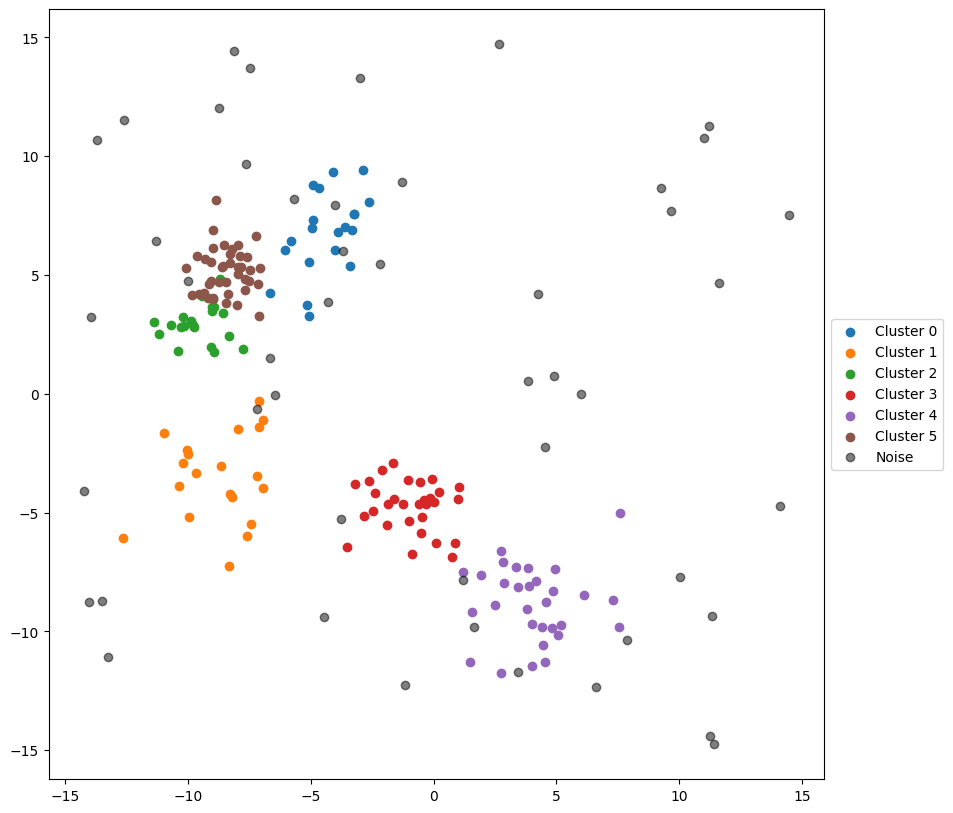
\includegraphics[width=0.9\linewidth]{Figures/dati_veri.png}
    \caption[Example of data for clustering]{Data points are coloured according to their label, while noise is shown in grey.}
    \label{fig:data_true}
\end{figure}

\noindent We are going to see the results of different clusterisation over the same data: \gls{kmeans}, \gls{gmm}, \gls{fcm}.
\paragraph{KMeans} We cluster the data using \gls{kmeans} with the correct number of centroids, i.e. $6$. In \cref{fig:data_kmeans} we can see that the noise has created an additional cluster and two of the original clusters have merged into one.
\begin{figure}[H]
	\centering
	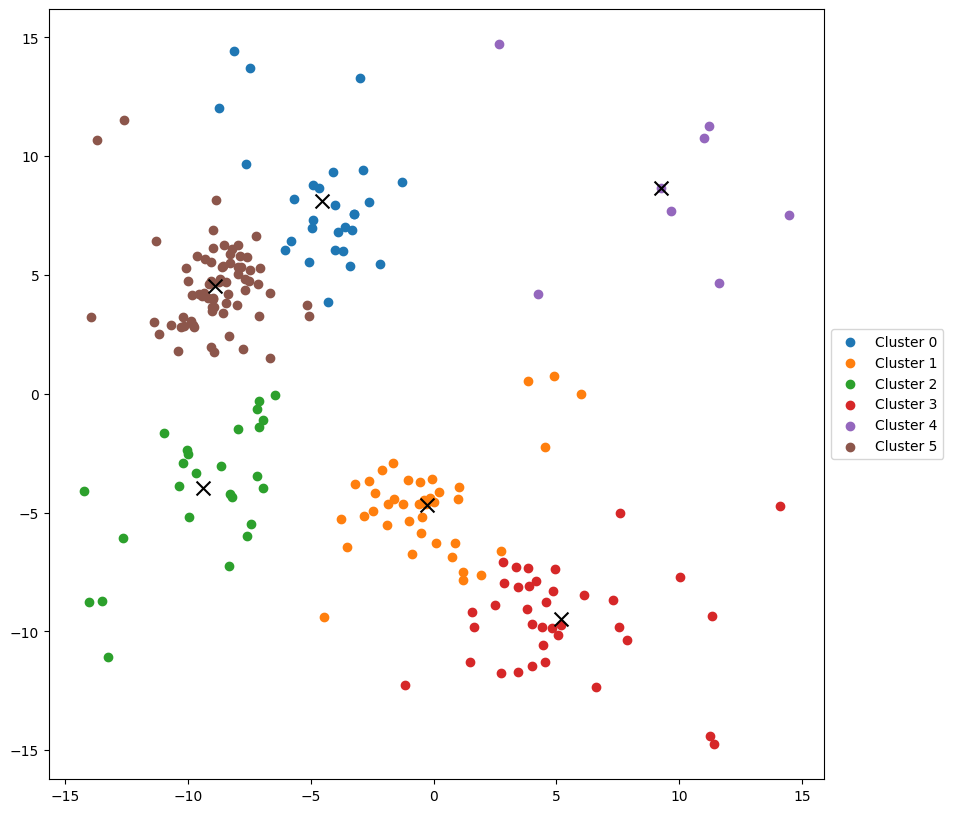
\includegraphics[width=0.9\linewidth]{Figures/dati_kmeans.png}
	\caption[Example of \gls{kmeans} clustering]{The data points are coloured according to the calculated label and the estimated centroid is indicated with an $\times$.}
	\label{fig:data_kmeans}
\end{figure}

\paragraph{GMM} Next, we apply clustering using a \gls{gmm} with $6$ centroids. In \cref{fig:data_gmm}, it can be seen that the cluster corresponding to noise has a very low weight, with a probability of $0.07$. Furthermore, the use of covariance matrices allows for a more precise determination of the centroid positions and provides additional information about the shape and spread of the clusters. This enables the identification of substructures or dependencies among clusters, which can be interpreted as a form of hierarchical organization. It is important to note that in \gls{gmm}, clusters are modeled as Gaussian distributions rather than discrete entities, meaning that what we observe are formal probability distributions rather than "real" clusters with strict boundaries.

\begin{figure}[H]
	\centering
	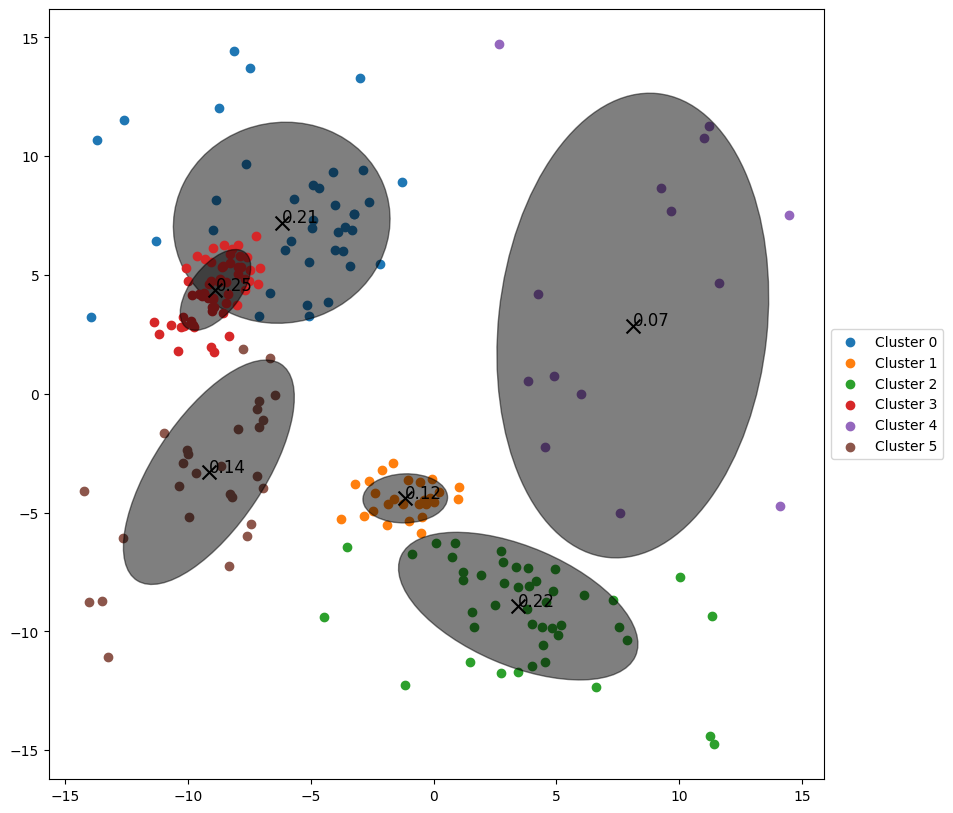
\includegraphics[width=0.9\linewidth]{Figures/dati_gmm.png}
	\caption[Example of GMM clustering]{The data points are coloured according to the Mahalanobis distance and the estimated centroid is indicated with an $\times$. The ellipse of the normal distribution represents the covariance and is a confidence region of $95\%$.}
	\label{fig:data_gmm}
\end{figure}

\newpage
\paragraph{FCM} Finally, let clustering be applied with \gls{fcm} using $6$ centroids. In \cref{fig:data_fcm} we observe that the centroids are less affected by noise, making it possible to identify which data are potentially noisy or shared between several clusters.

\begin{figure}[H]
	\centering
	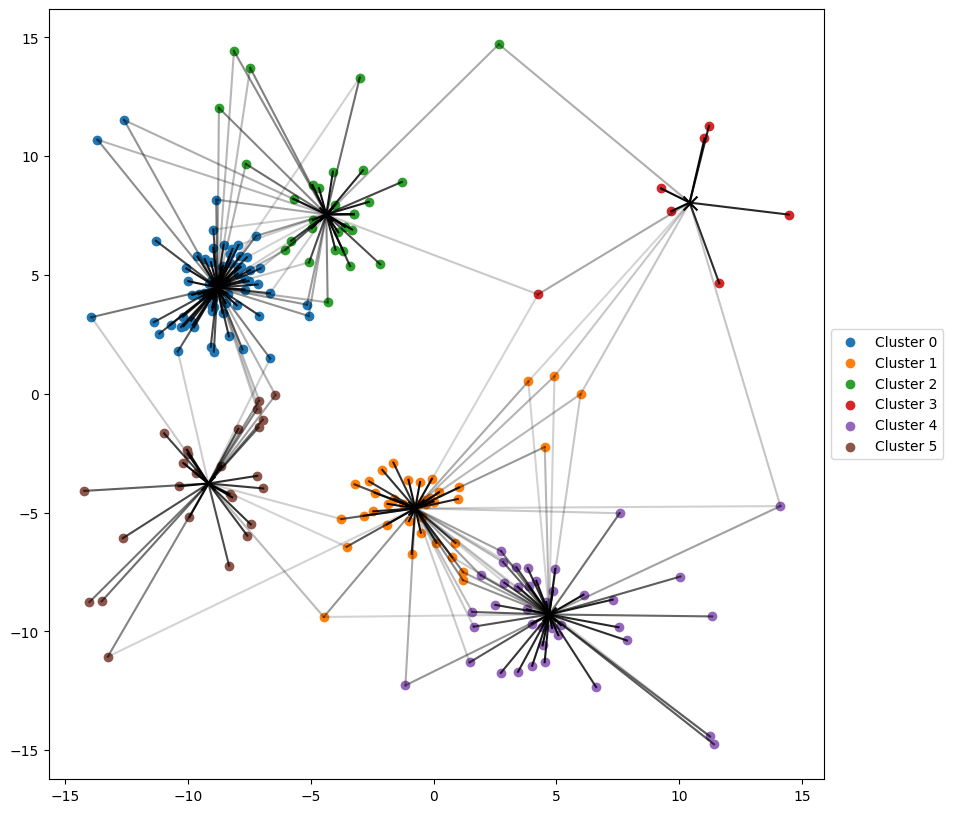
\includegraphics[width=0.9\linewidth]{Figures/dati_fcm.png}
	\caption[Example of FCM clustering]{The data points are coloured according to the most probable label and the estimated centroid is indicated with an $\times$. The lines indicate the assignments with the greatest degree of affiliation of each point to the clusters; the darker the lines, the stronger the assignment.}
	\label{fig:data_fcm}
\end{figure}

\bigskip
\noindent We have observed that in the presence of noise, the algorithm \gls{fcm} can be very useful due to its flexibility in handling overlapping clusters and noisy data. On the other hand, the algorithm \gls{gmm}, while providing valuable insights about the nature of the data through its probabilistic framework, is computationally expensive, especially for large datasets or high-dimensional spaces. In this thesis, we prioritize computational efficiency and scalability. Therefore, we use the \gls{fcm} algorithm to reduce the amount of information to be processed, leveraging its ability to model uncertainty in cluster assignments, and the \gls{kmeans} algorithm for efficient initialisation of centroids.
